\chapter{Introduction}
\label{chap:introduction}

\section{Bilateria lineage}
Cerebral bilateral symmetry is a universal quality of organisms belonging to the Bilateria lineage \cite{Concha2012}\cite{Corballis2009}, the phylum incorporating all species with a single plane of symmetry, in contrast with their sister group, Cnidaria (\autoref{fig:bilateriaphylum}). Bilateral symmetry is a byproduct of the activity of two separate developmental processes, that produce two axes of polarity \cite{Finnerty2003}, and therefore a symmetry plane; the formation of a primary body axis, that corresponds to the long anatomical dimension of the animal, called \acf{rc} (i.e. head-to-tail), primarily dictated by highly conserved controlled activation of HOX genes during cell differentiation; the shaping of a secondary body axis, orthogonal to \ac{rc}, named \acf{dv} (i.e. back-to-front), attributed to a variety of genes,  such as the chromatin organizer CTCF, the left-right determination factor Nodal and central HOX genes \cite{Heger2020}.  For the mammals group, the brain is anatomically divided into a left and right hemisphere.  Another important bilateria common characteristic is the germ line \textbf{triploblasticity}: the embryo begins as a flat disk with three distinct cell layers called \textbf{endoderm}, \textbf{mesoderm}, and \textbf{ectoderm}. Of significance in the neural system formation is the ectoderm, which is initially equivalent to one of the flat disk sides. Shortly after conception, the disk folds, in a way that the ectoderm side forms a tube-like shape, named \textbf{neural tube}, which acts as the neural system precursor, under a process called \textbf{neurulation}. All bilateria exhibit a \ac{cns}, which entirely develops from the neural tube walls \cite{F.Bear2016a}. Next pivotal step in the brain development, \textbf{differentiation}, leads to the creation of three distinct compartments along \acf{rc} axis, the \textbf{forebrain}, which develops into the brain cerebellum, the \textbf{midbrain}, and the \textbf{hindbrain}, which gives rise to the spinal cord in vertebrates. Until this stage, perfect bilateral symmetry is observed in the \ac{cns}. [CITATION NEEDED] Because of the highly diverse mechanisms acting on bilateria subgroups after this developmental step of \ac{cns},  the focus is subsequently directed on the vertebrates case. 


\section{Neurogenesis}
The cells comprising the neural tube are named \textbf{neuroepithelial}, and exhibit similar properties with stem cells, that is limited multipotency (i.e. they can differentiate into multiple cell types) and limited self-renewing (i.e. they can divide symmetrically into new neuroepithelial cells a finite number of times) \cite{Gotz2005}, while also properties of epithelial cells, that is polarity (i.e. asymmetrical cellular organization, with distinct basal and apical surfaces) and attachment (i.e. junctions connect adjacent cells) . After anatomical differentiation, self-renewing is activated, leading to cells proliferation and \ac{cns} bilateral expansion, while attachment is hindered, gradually exchanging the neuroepithelial cells with \textbf{radial glial (RG) cells}, the fate-restricted progenitors of neurons, marking the initiation of \textbf{neurogenesis}.\cite{Gotz2005}

Among a set of common properties, a

At the early developmental stages, the brain precursor





 



Phenomena, such as the asymmetric cell division of neuroblasts for the proteostoma case and of radial glial cells for the vertebrate case \cite{Bailly2013} , or the neuroblasts (i.e. neural stem cells) unilateral programmed migration  in vertebrates, asymmetric fluid flow   by motile cilia-generated hair-like i.e. cell organelles with the ability to beat) \cite{Grimes2017}, generate a solid basis for asymmetry presence in the \ac{cns}, implying different cell ratios of similar types on each \ac{dv} side \cite{Concha2012}. Cerebral bilateral symmetry therefore begins breaking down during fetal development, with the results in humans being anatomically visible (\autoref{fig:brainlat}). This fact gives rise to partial functional disassociation, called brain lateralization, the differential activation of each hemisphere for subsets of tasks. Lateralization becomes visible when examining organisms' behavior, with the most studied trait in humans being handedness and language \cite{Schmitz2019}\cite{Corballis2009}. 
Along with the purely genetic reasons, environment also plays a significant role in affecting cerebral bilateral asymmetry. How the environmental effect manifests itself though differs across species, with the primary reason being that neurogeneration is quite limited in humans during adulthood, with a high percentage of neuroblasts unable to migrate long distances or survive, a case that does not hold, for example, for rodents \cite{Ernst2015}. There has  


\begin{figure}
	\centering
	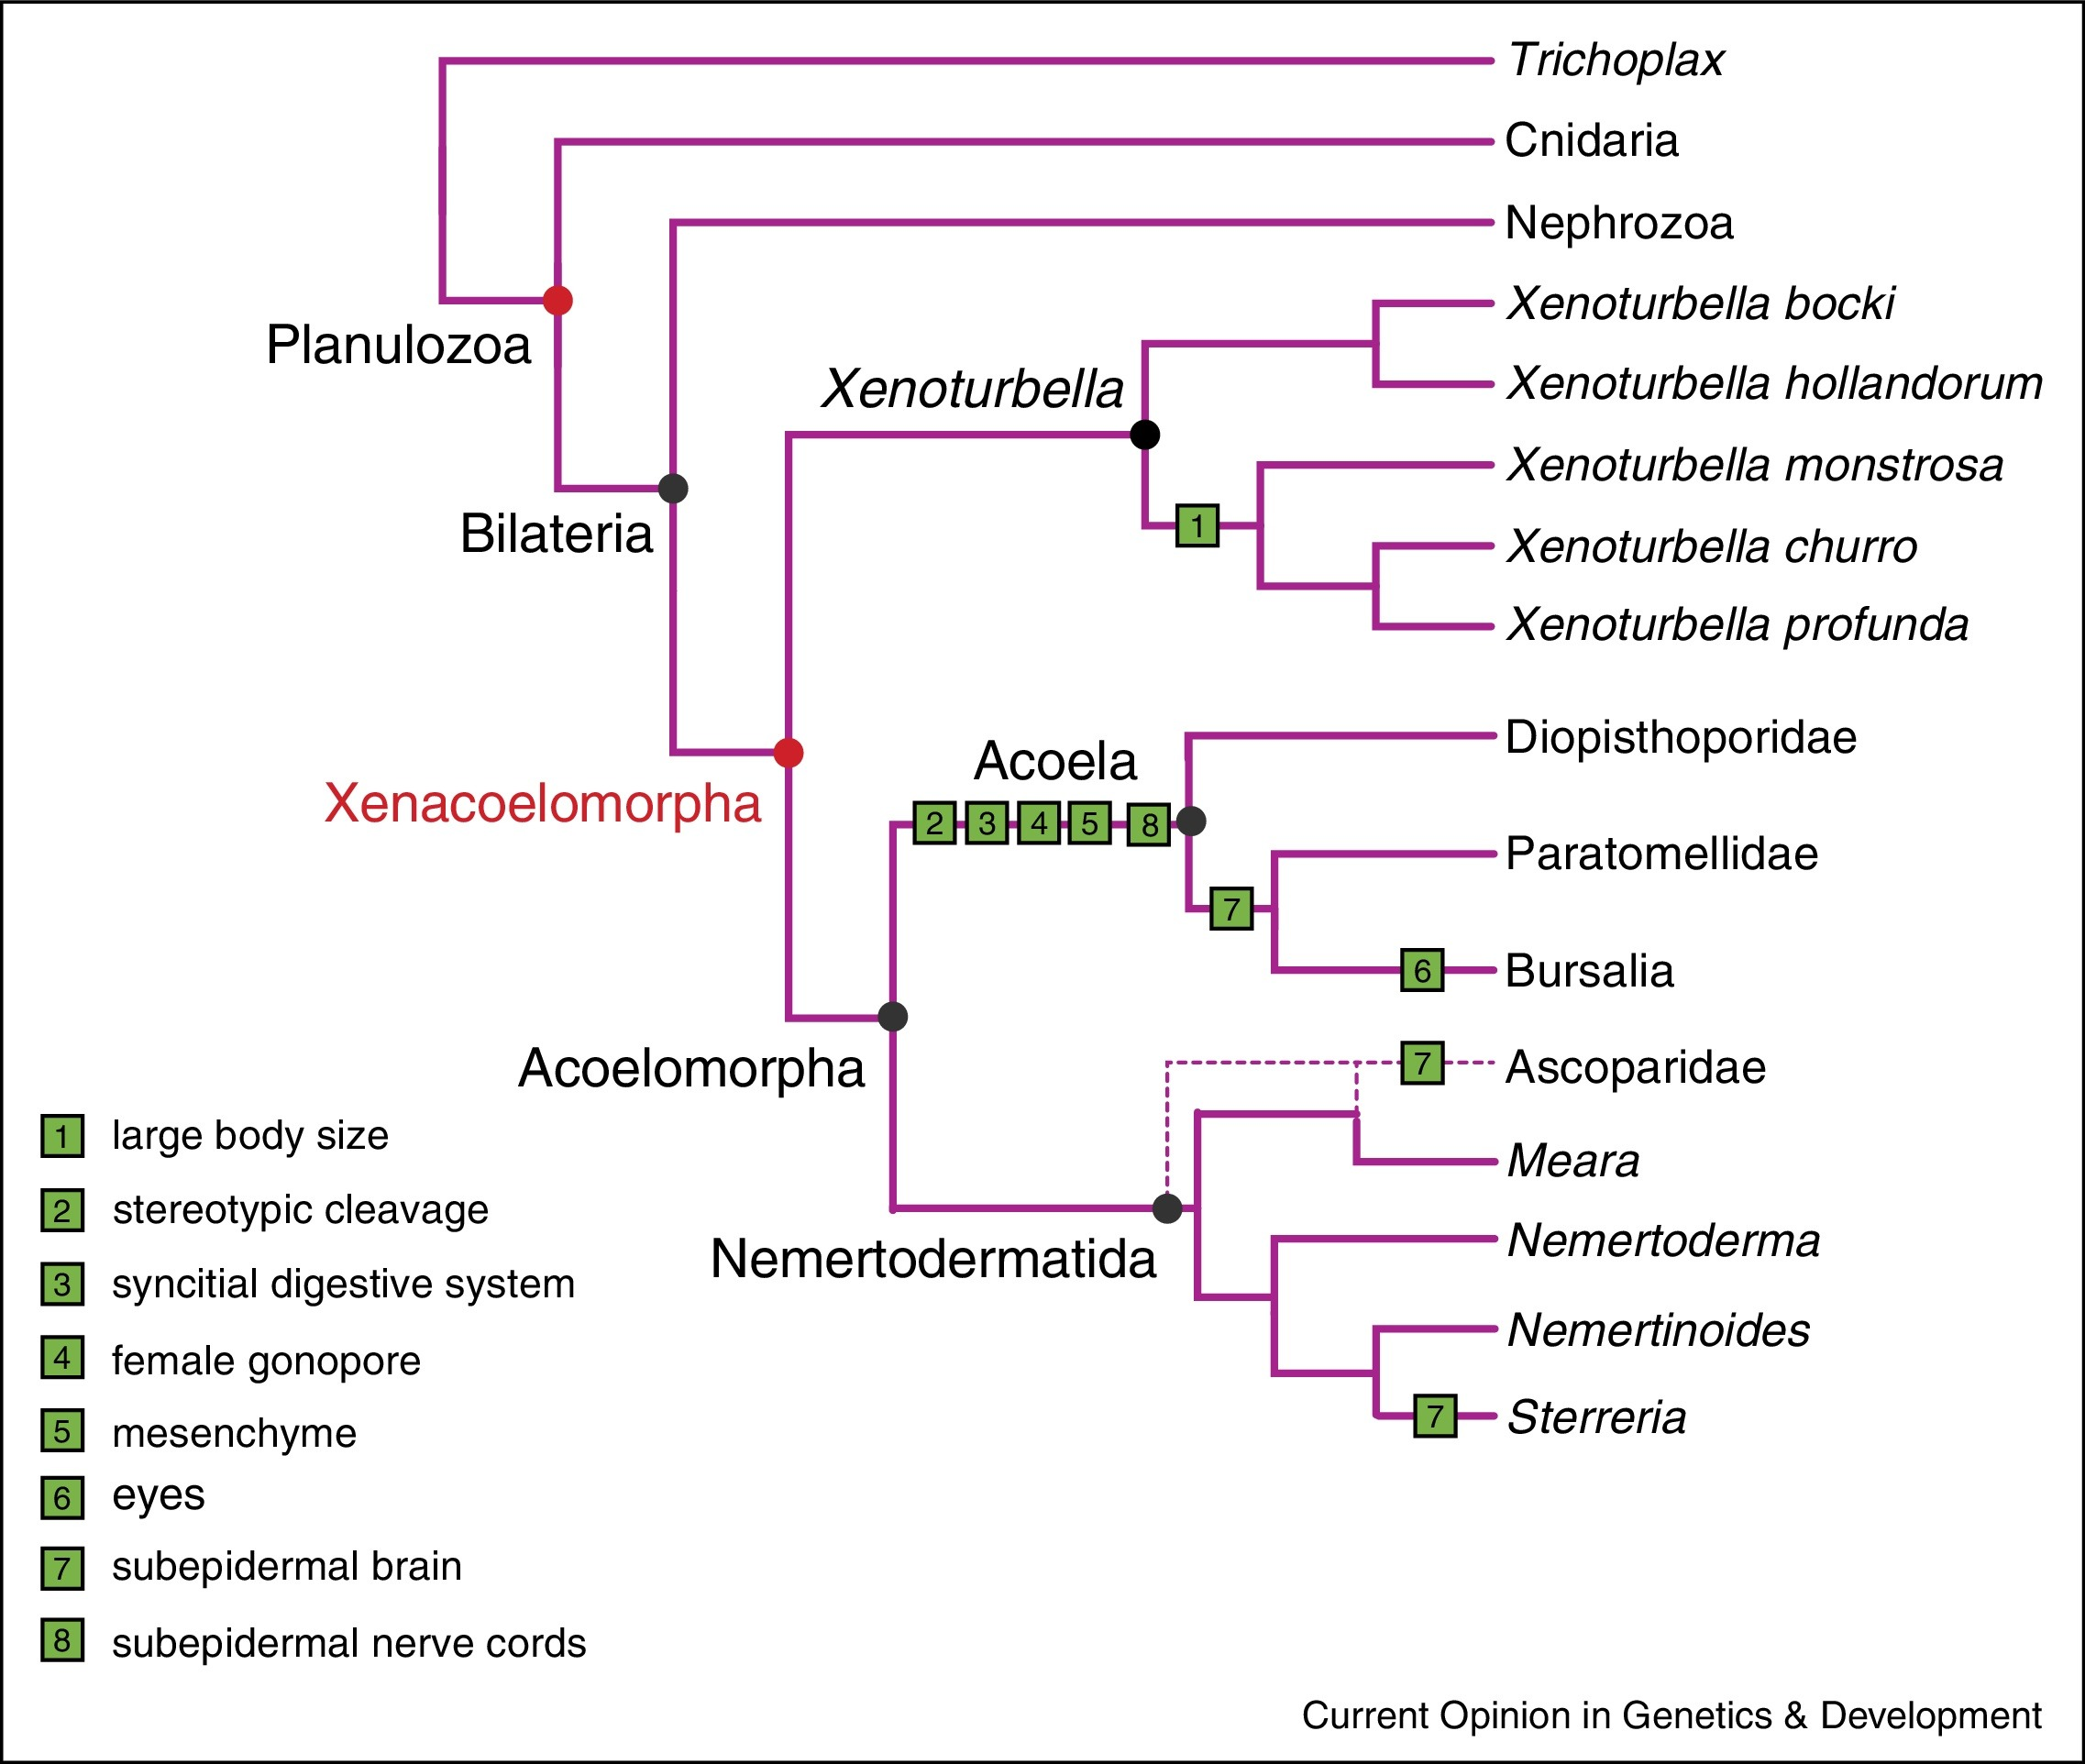
\includegraphics[width=0.7\linewidth]{bilateria_phylum}
	\caption[Bilateria clade \cite{Hejnol2016}]{Species phylogenetic tree subset, displaying bilateria clade, its sister clade, Cnidaria, and the direct children\cite{Hejnol2016}. Of great importance on the evolutionary studies of bilateral symmetry is the Xenacoelomorpha clade.}
	\label{fig:bilateriaphylum}
\end{figure}

\begin{figure}
	\centering
	\includesvg[width=\textwidth]{da_visualization}\\
	\caption[Illustration of brain asymmetry]{Illustration of brain asymmetry. Normalized differences of the distances of landmarks from the center of mass of each averaged hemisphere midthickness surface, after a scaling and alignment process, across the studied population.}
	\label{fig:brainlat}
\end{figure}

\section{Phenotypic trait analysis}
\subsection{Summary on cortex anatomy}
 
\subsection{Dataset Description}
 
\subsection{Shapes Normalization}
\Ac{mri} output is affected by the subject positioning and technical error.  Volumetric differences also increase the level of discrepancies among \ac{mri} samples. To remedy positioning and volume deviations, a normalization is required, achieved by projecting each subject onto \textbf{Kendall shape space} \cite{Klingenberg2020}. TO BE CONTINUED

 
\subsection{Asymmetry Components}
TO BE CONTINUED
Of primary interest in this work is \ac{da}, the asymmetric component that arises by comparing a single individual's hemispheric surfaces landmarks differences, computed through a process of alignment, reflection and subtraction of the landmarks pairs. \ac{da} captures information about anatomic characteristics, such as the overall counterclockwise torque, named `Yakovlevian torque' \cite{LeMay1976}, that is observed in humans between the right and left hemisphere (\autoref{fig:yaktorque}). Past studies have shown that abnormal \ac{da} may be an indication of certain diseases. The lack of it may imply schizophrenia predisposition \cite{Ribolsi2014}. Any significant abnormalities may be indicative of other psychiatric disorders, such as autism or developmental language disorder \cite{Herbert2005}\cite{Kong2022}. 

\subsubsection{Statistical analysis}
Bilateral asymmetry is mainly described using three components in literature \cite{klingenberg2002}\cite{Vingerhoets2021}; \acf{da}, the focus of this study, corresponds to the hemispheric side effect; antisymmetry, which is related to the effect where sidedness is random in a population (i.e. left-right randomly switches to right-left), is not observed in the human cerebral cortex, in contrast to other internal organs positions, or organisms \cite{Neubauer2020}; \acf{fa}, encompasses any random developmental and environmental effects, that cannot be explained with the existing knowledge. The observed deviations can be statistically linearly modeled as products of two effects, the hemisphere side studied and the individual specimen analyzed, as well as their interaction \cite{klingenberg2002}. Formally, based on \cite{VanDongen1999} assuming the presence of replications of the observation per individual, to account for technical error, a mixed linear model representing the aforementioned dependencies is defined as:
\begin{equation}
	Y_{ijk} = \mu + \beta + I_i + S_{ij} + E_{ijk}
\end{equation}
where $Y_{ijk}$ is the phenotype of the i-th individual, from the j-th side, under the k-th replication, $\mu$ and $\beta$ are the fixed intercept and fixed side effect respectively, $I_i\sim\mathcal{N}(0,\sigma^2_{ind})$ is the random individual effect,  $S_{ij}\sim\mathcal{N}(0,\sigma^2_{FA})$ is the random side and individual specific effect, matched to \ac{fa}, and $E_{ijk}\sim\mathcal{N}(0,\sigma^2_{ME})$ is the measurement error. Replications are necessary in such a study, in order to differentiate \ac{fa} effect from the measurement error. Given this definition, a way to measure the statistical significance is through an F-test applied on 2-way \ac{anova}, to relate the \ac{rss} ratios of effects to observable error terms, and of fluctuating effect to the measurement error. Extra care needs to be given on the determination of the \ac{dof} of each term, given the preprocessing applied to bring the hemispheres surfaces into Kendall shape space. Those are extracted from the rigorous work in \cite{klingenberg2002}. Given that the analysis is performed on a pair of symmetric objects, and not on a single symmetric object, this configuration is named matching asymmetry analysis. In order to avoid further de facto assumptions, regarding the distribution of TO BE CONTINUED
\subsection{Phenotypic partitioning}\label{sec:hsc}
\Acf{hsc} is an unsupervised method of iterative partitioning, that makes use of the distance matrix eigenvectors \cite{Ng2002}. It results into a binary tree structure (i.e. each parent shape is partitioned into two children). In the current study, a level-4 partitioning is performed, resulting into 31 partitions. Subsequently, they are transformed to the corresponding principal components that explain 80\% of the variance, for reasons of further dimensionality reduction. TO BE CONTINUED


\begin{figure}
	\centering
	\includesvg[]{torque0510}
	\caption[Illustration of the Yakovlevian torque]{Illustration of the Yakovlevian torque. Displayed by a red line rotated counterclockwise 0.51 degrees in relation to the perfectly vertical black line, as calculated by using the average angle of the longest edges (in blue) of the convex hulls of the horizontal plane projection of each hemisphere midthickness surface, after a scaling and alignment process, across the studied population.}
	\label{fig:yaktorque}
\end{figure}

\section{Breaking the complexity into parts}
TO BE EXPANDED

The present work evaluates the brain asymmetry genetic landscape in a coarse-to-fine segmentation, through the application of \ac{hsc}\cite{Ng2002}, discussed in \autoref{sec:hsc}. The technique has been used in a number of different related studies \cite{Claes2018}\cite{Naqvi2021}, yielding results that are in accordance with the underlying anatomic features. The main reason behind this partitioning is the intrinsic complexity of the studied phenotype, eliciting expected differences in the genomic profiles of each cerebral cortex region. The basic assumption made is that topologically close landmarks share similar genetic background. In general though, this type of distance-based clustering is governed by the least quantity of assumptions, regarding the shape or form of the cluster \cite{VonLuxburg2007}. The partitions' genetic juxtaposition is valuable for identifying which regions share similar significant genetic loci, highlighting the corresponding genes contribution, or showcasing the specialization of certain regions that share little to no similarities with their neighbors. Identifying the latter provides a way of mapping the developmental activation of each locus, bringing forth the opportunity to augment the results of related developmental studies \cite{Vijayakumar2016}.

\section{Searching for the origin}
TO BE EXPANDED

The genomic studies are performed under the framework of \ac{snp}-by-\ac{snp} \ac{cca}. The goal is to incorporate multi-allelic \acp{snp} and, more importantly, multivariate phenotype, in a single hypothesis test per \ac{snp}, that is whether the phenotype is significantly correlated with each analyzed \ac{snp}. In general, there is an abundance of strategies on how to perform multivariate \ac{gwas}, ranging from direct methods, that approximate the inputs relation either in an unbiased manner or making certain educated guesses, to more complex techniques, that increase statistical power by transforming the inputs, at the expense of explanatory ability \cite{Galesloot2014}. There are also methods that are based on the meta-analysis of outcomes from univariate studies, commonly used to juxtapose experiments from separate sources, for which the original data is absent or the exact replication of the study is arduous \cite{Cichonska2016}. Which approach performs best mainly lies on the dataset properties and the nature of the scientific question. Factors such as low sample size \cite{Sheng2021}, genes pleiotropic effects \cite{Fernandes2021} or within-study variation \cite{Jackson2011} tend to handicap the statistical modeling and increase the type I and II errors of the corresponding hypothesis tests. In this study, \ac{cca} was primarily chosen due to the high capacity in efficiently reducing the inputs dimensionality while preserving most information regarding their correlation. Diverse experiments, analyzed in \autoref{chap:gwas}, have been applied to identify the method that gives high fidelity results, consistent with relevant literature. The analysis outcome requires further processing, as explained in \autoref{sec:postprocessing}, to account for the main weakness of this method, that it does not consider the \ac{snp}-to-\ac{snp} effect, tackled using as proxy the notion of \ac{ld}, and subsequently to topologically and functionally enhance the filtered findings. Once this additional step has been performed, a cross-traits analysis is applied, described in \autoref{sec:metaanalysis}, where the \ac{da} genetic signature is compared with the signatures of phenotypic traits, analyzed in a similar study \cite{Naqvi2021}, the cerebral and facial shapes.


\section{Data description}
In this study, targeted on humans, a cross section between the dependent cerebral asymmetry and the independent genetic factors is performed, in an effort to discover affiliated genetic regions and provide a novel understanding of the related genes cooperation. With the advent of technology capable to collect and process genomes from different individuals in relatively high speed, vast databases have been constructed. One of the main players in the data collection has been UK Biobank; a large-scale database from a randomized consortium of 500,000 individuals, whose genome has been collected, from whom  48,000 subjects had also participated in brain \ac{mri} collection process, as of December 2020 \cite{Littlejohns2020}. In this thesis, we exploit this newly acquired dataset to identify the key loci that are related to the human brain surface symmetry. Only healthy self-proclaimed white European individuals were considered. 

\section{Novelties based on related literature} 
 Due to the biological importance of cerebral bilateral asymmetry, it is a subject that has been rigorously studied from multiple viewpoints.
 \subsection{Evolution}
 From an evolutionary stand, it is extremely rare for the right conditions to occur, in order for any soft tissue specimen to be preserved, across a considerable amount of time. The only known way is through mineralization \cite{Purnell2018}. This fact renders a mammal's ancestor brain almost impossible to retrieve. Nevertheless, endocranial imprints have been used as a proxy to describe the relationships between hominids and their ancestors \cite{Balzeau2012}\cite{Neubauer2020}. The reason behind this phenotypic delegation is purely practical. The brain size and shape follow the container volume restrictions. The brain sulci (i.e. grooves) and gyri (i.e. bumps) in humans are the result of the tremendous expansion of the cerebral cortex surface area during fetal development, folding and wrinkling in order to fit the skull \cite{F.Bear2016}. Although such studies support the theory of propagating asymmetry among studied individuals, with the most evident signs of \ac{da} in human skulls, little information about the surface shape can be retrieved, as only the convex hull shape of the brain can be delineated from such process. Through the association of brain asymmetry with \acs{dna}, a universal code among organisms, it becomes possible to deploy tools used by evolutionary geneticists, to identify the phylogenetic tree of this complex trait, locating conserved regions among organisms and their predicted divergence in time, under a pleiotropic model \cite{Koch2021}.
 \subsection{Clinical studies}
 